\documentclass[11pt]{article}

\usepackage[margin=1.1in]{geometry}
\usepackage{graphicx}
\usepackage{booktabs}
\usepackage{amsmath}
\usepackage{microtype}
\usepackage[hidelinks]{hyperref}
\usepackage{caption}
\captionsetup{font=small, labelfont=bf, width=0.92\textwidth}
\graphicspath{{../}}

\title{\textbf{Psychedelic Therapy as Precision-Modulated Exposure:\\
Preregistered Simulations of Avoidance, Capture, and Entrenchment}}
\author{Joshua Rogers\\ \small Independent researcher \\ \small \texttt{josh@envitae.io}}
\date{August 2026 \\ \small Preprint draft. Companion to ``What the Theory Never
Specifies.'' Comments welcome.}

\begin{document}
\maketitle

\begin{abstract}
\noindent A companion paper found that in the minimal Bayesian model family both
REBUS and ALBUS describe, belief strengthening (SEBUS) emerges from precision
mechanics nowhere and from avoidance of a costly diagnostic test everywhere it
appears, with prior relaxation acting to make the avoided test worth running. That
result converges with a thirty-year-old clinical account: safety behaviors maintain
threat beliefs by preventing disconfirmation, and exposure works by arranging the
missing test. This paper composes the mechanisms, all preregistered in a public
git history, and asks the clinical questions: when does a session help, when does
it entrench, and what makes a belief chronic. Five results. First, a session's
effect is gated by a three-dimensional window: dose must clear a cost-dependent
crossover, cost must sit below a ceiling, and integration must capture the state
after the avoided test has run; missing a coordinate entrenches the belief or
dissolves it without replacing it. Second, ALBUS's own gain mechanism, implemented,
cannot strengthen a belief against a freely run test and cannot entrench without
avoidance; the two SEBUS accounts separate behaviorally by the sign of the
low-dose change in diagnostic engagement, and active drug-added strengthening
exists only where gain and avoidance combine, a confirmed interior dose window.
Third, replacing consolidation with hierarchical parameter learning does not
dissolve the underdetermination identified in the companion paper; it inherits it,
and it surfaces a new mechanism, interpretive capture, in which ambiguous evidence
is encoded as confirmation. Fourth, across repeated sessions capture alone is
delay, not destiny: in a world that keeps generating disconfirming evidence, the
sealed belief leaks and recovers. Fifth, composing capture with avoidance closes a
ratchet that nothing else closed: conviction climbs session over session and locks
permanently, because avoidance starves the belief of its test while capture
prevents the stored doubt that would otherwise reopen it. Treatment then fails in
three distinct ways, each with an observable signature in diagnostic engagement.
We claim convergence with the exposure account, not discovery of it; the
formalization contributes necessity results, a derived drug mechanism, and
discriminating predictions the verbal accounts do not fix.
\end{abstract}

\section{Introduction}

The companion paper \cite{rogers2026} implemented REBUS \cite{carhart2019} and
ALBUS \cite{safron2025} as stated and reported three findings: literal REBUS
produces no lasting change because dose enters only through a precision that
reverts; a consolidation process rescues persistence but four defensible readings
of what it operates on disagree about whether the drug matters at all; and SEBUS,
ALBUS's low-dose belief strengthening, emerges from no precision mechanism tried
and from exactly one non-precision mechanism: pricing the single diagnostic test
so that the agent declines to run it.

That last result is not new as an idea. It is the clinical safety-behaviors
account \cite{salkovskis1991}: threat beliefs persist because the behaviors they
motivate prevent the disconfirming test, which is why repeated benign experience
fails to teach, and why exposure therapy works by arranging the missing test
\cite{foakozak1986,craske2014}. Wolff and colleagues \cite{wolff2020} proposed
verbally that psychedelic belief relaxation enables episodes of relatively
avoidance-free exposure, and prospective data show post-psychedelic reductions in
experiential avoidance tracking clinical improvement \cite{zeifman2020avoid}. The
convergence suggests a specific reading of psychedelic therapy: the drug is a
precision intervention on an exposure problem. This paper takes that reading
seriously and asks what follows when the mechanisms are composed: relaxation,
avoidance, biased learning, and repetition across sessions.

Every arm was declared in a written amendment committed to git before its code
existed, continuing the companion paper's protocol; the final confirmatory
amendment was additionally pushed to a public repository before running, giving
it a third-party timestamp. Failed predictions are reported alongside confirmed
ones, and two of this paper's central negative results were declared as live
possibilities before their arms ran.

The contributions:

\begin{enumerate}
  \item \textbf{The therapeutic window is three-dimensional} (Section~\ref{sec:window}).
  Dose must clear a cost-dependent crossover, cost must sit below a ceiling, and
  integration must capture the post-test state. Missing any coordinate makes the
  same session entrench the belief or dissolve it without replacing it.
  \item \textbf{ALBUS's gain mechanism, implemented, needs avoidance too}
  (Section~\ref{sec:gain}). It cannot strengthen a belief against a freely run
  test at any strength tried, cannot entrench after integration without a test
  cost, and combines with avoidance to produce the one regime of active
  drug-added strengthening, an interior dose window confirmed under a declared
  replication. The two SEBUS accounts separate by the sign of the low-dose change
  in diagnostic engagement.
  \item \textbf{Learning inherits the fork, and perception adds capture}
  (Section~\ref{sec:learning}). Replacing consolidation with hierarchical
  parameter learning reproduces the companion paper's underdetermination in the
  framework's own vocabulary, and top-down weighted encoding yields interpretive
  capture: ambiguous evidence encoded as confirmation, freezing learning within a
  session.
  \item \textbf{Chronicity is a composition phenomenon}
  (Sections~\ref{sec:sessions} and \ref{sec:ratchet}). Capture alone delays
  recovery by a factor of three to six and cannot prevent it. Avoidance alone is
  self-limiting: it stores up the doubt that eventually reopens the test.
  Composed, they close a ratchet that entrenches permanently, and treatment fails
  in three distinct, behaviorally separable ways.
\end{enumerate}

Nothing here bears on phenomenal experience; everything is belief dynamics. And
the framing claim is bounded: we assert convergence with the exposure account,
not discovery. The formalization earns its place through what the verbal accounts
leave open: necessity (which mechanisms cannot produce the phenomena), a derived
rather than posited drug mechanism, and quantitative predictions.

\section{Related work}
\label{sec:related}

The clinical line is primary for this paper. Safety-seeking behavior maintains
threat beliefs by preventing disconfirmation \cite{salkovskis1991}; exposure is
the deliberate arrangement of corrective information \cite{foakozak1986}, with
modern treatments framing it as inhibitory learning under maximized expectancy
violation \cite{craske2014}. Wolff and colleagues \cite{wolff2020} connected this
to psychedelics with a verbal model on which relaxation enables avoidance-free
exposure; Zeifman and colleagues \cite{zeifman2020avoid} supply prospective data
linking reduced experiential avoidance to symptom change. The computational
psychosis literature models belief maintenance through aberrant precision
\cite{corlett2010,adams2013,sterzer2018} and hallucination through strong priors
\cite{powers2017}; the avoidance route and its composition with precision are, to
our knowledge, not implemented there. The persistence question for psychedelics
is posed empirically by \cite{zeifman2025}. The companion paper
\cite{rogers2026} contains the model family, the preregistration protocol, and
the baseline results this paper composes; its own related work covers the
simulation literature \cite{rajpal2022,sandved2021,fisher2024,mago2026}.

\section{The model family, briefly}
\label{sec:model}

Full specifications are in the companion paper and the repository; what follows
is the minimum to read the results. Six hypotheses; hypothesis 0 true, hypothesis
1 the maladaptive conviction, held at prior conviction 0.8007 unless stated. The
\textbf{acting agent} chooses among seven probes by epistemic value with softmax
precision 8: six shallow probes that can eliminate irrelevant alternatives but
never separate 0 from 1, and one deep probe that does, whose value can carry a
cost. Dose relaxes the weight on the stored prior by $(1-d)$ during a session of
14 decisions. The \textbf{learning layer} stores the prior as a probability
vector with count mass $N_0 = 20$ and updates it with mass $E = 10$ of a
normalized increment per session; increments are computed from the window-end
posterior, from likelihood-only evidence, or from stepwise interpretations
weighted by the current belief raised to $\kappa$ (capture, at $\kappa = 3$;
exact at $\kappa = 1$). A \textbf{two-level perceptual variant} (context, events,
observations) grounds the capture rule; under exact inference it reduces to the
flat model. Consolidation, where used, is the arithmetic mixture of the companion
paper at $c = 0.8$. All sweeps are paired: observation draws are shared across
dose and mechanism, so exact zeros are exact.

\section{The therapeutic window}
\label{sec:window}

Composing the costly-test agent with consolidation applied at a swept time $t_c$
inside the session (amendment 6, predictions 24 to 26) gives the clinical
geometry. The lasting-conviction crossover sits at the acute SEBUS crossover
measured in the companion paper (0.25 versus 0.23 at cost 0.3; 0.45 versus 0.42;
0.55 versus 0.50) and is robust to consolidation strength: below it, integration
locks in the session's inflation and the session entrenches; above it, the
session helps. Above the cost ceiling, conviction and insight dissociate: high
dose still drags lasting conviction below baseline by pure dilution while lasting
insight stays at 0.001, because the deep test never runs and no discriminating
evidence exists to lock in. Timing adds the third coordinate: the within-session
conviction trajectory rises first (shallow-probe elimination inflates by
redistribution) and falls only once the deep test runs, so consolidating
mid-session captures the inflation peak, and consolidating early captures
dilution but no learning (lasting insight 0.003 at $t_c = 4$ against 0.130 at
$t_c = 14$, cost 0.3, dose 0.5). Dose never adds lasting conviction anywhere in
the grid (4,200 paired comparisons, maximum excess $-0.0046$).

\begin{figure}[t]
\centering
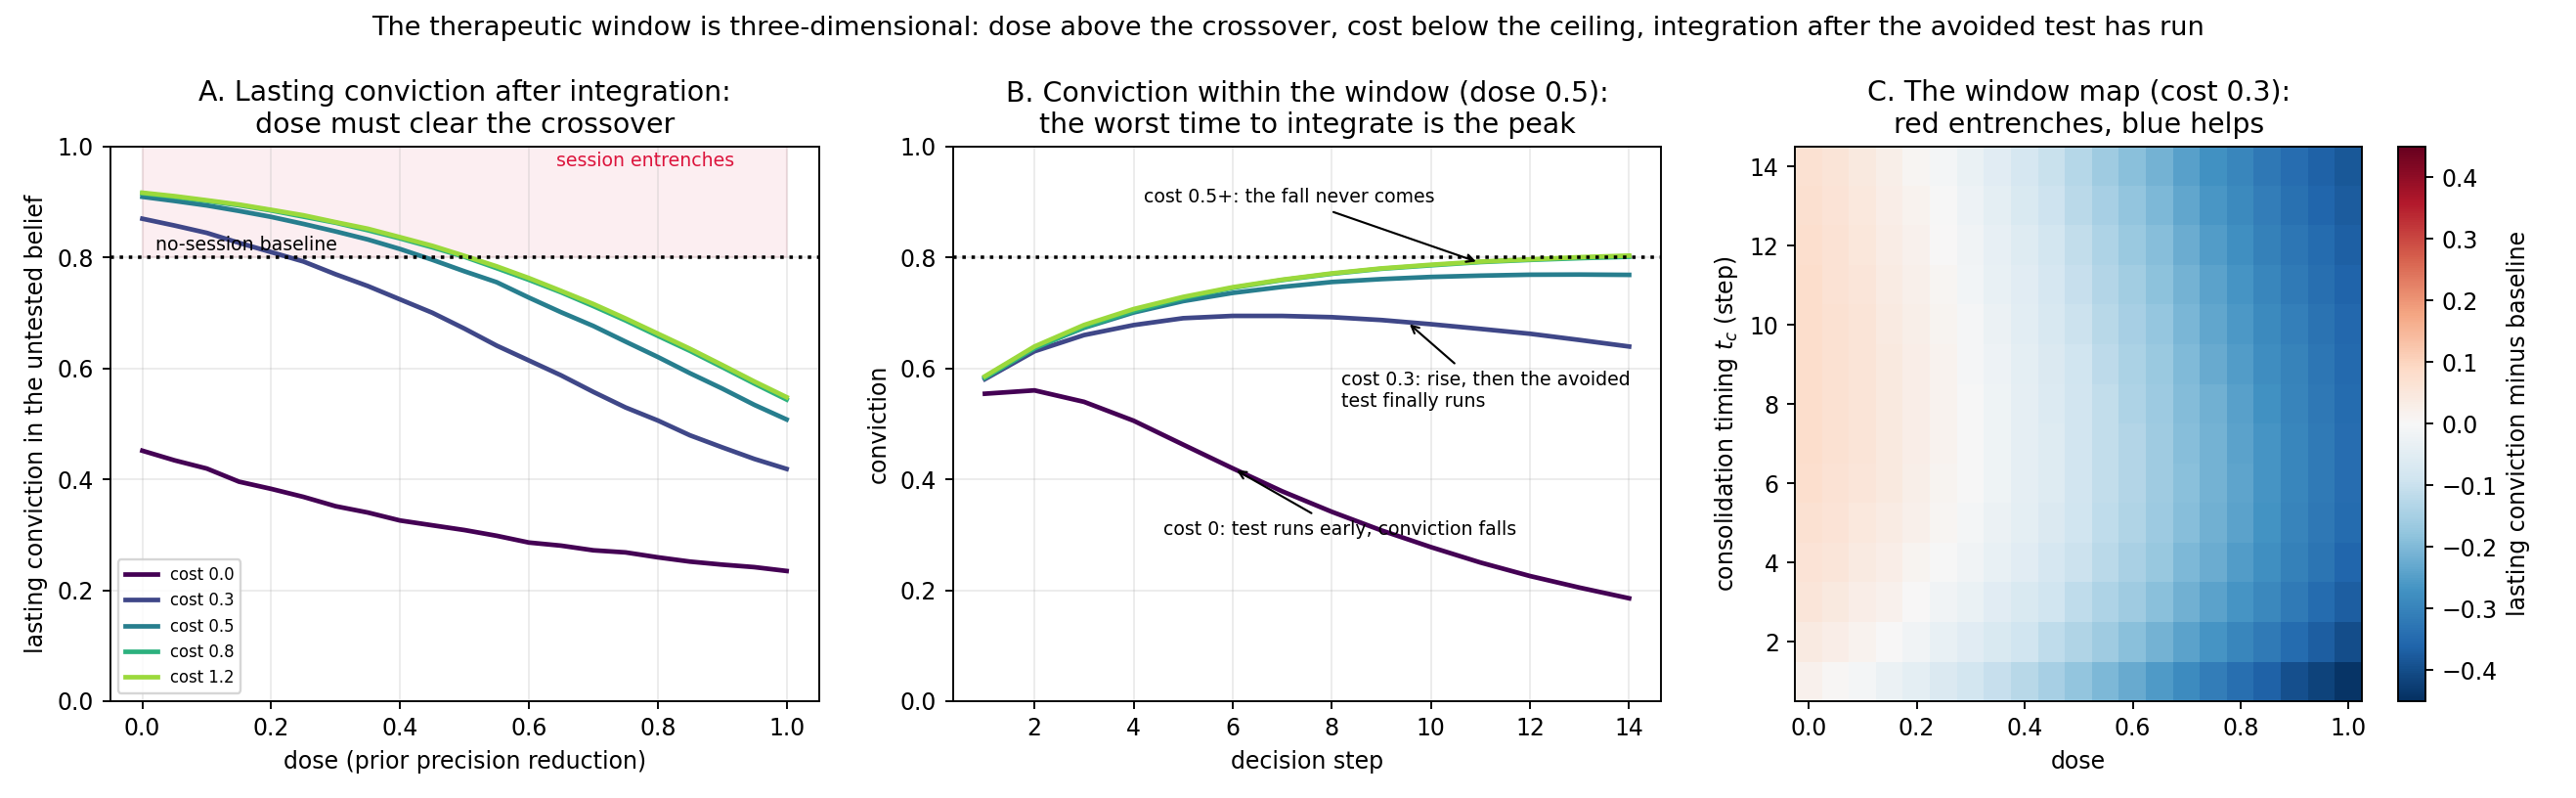
\includegraphics[width=\textwidth]{figure_window.png}
\caption{The therapeutic window. (A) Lasting conviction by dose and cost after
integration; the crossover gates benefit. (B) Within-session conviction:
integration timing decides what gets locked in. (C) The window map over dose and
timing: red entrenches, blue helps.}
\label{fig:window}
\end{figure}

\section{Gain versus avoidance}
\label{sec:gain}

ALBUS's own proposed mechanism is a low-dose gain increase on priors. The
companion paper excluded it deliberately, since building it in produces SEBUS by
construction; the informative move is to implement it beside the avoidance
account and find the discriminators (amendment 7, predictions 27 to 29). The
mapping $\gamma(d) = \gamma_0 (1-d)(1+Ad)$ nests the REBUS mapping at $A = 0$ and
gives a low-dose gain peak for $A > 1$ (factor 1.56 at $A = 4$).

Three results. First, with a free diagnostic test, window-end conviction never
exceeds the pre-dose baseline at any gain and any dose (peak 0.63 at $A = 4$
against 0.80): an agent that can cheaply check its belief still checks it, and
two or three checks beat a 1.56-fold boosted prior. Gain also never entrenches
after integration without a test cost. Even under ALBUS's own mechanism,
avoidance remains the load-bearing quantity. Second, the accounts separate by
sign: under gain with a free test, diagnostic engagement at low dose falls below
its sober value (0.239 to 0.200 at $A = 4$); under avoidance it never falls and
rises with dose. The sign of the low-dose change in diagnostic engagement is a
behavioral discriminator a task battery could target. Third, gain amplifies
avoidance: the SEBUS dose region at cost 0.3 grows from width 0.23 at $A = 0$ to
0.80 at $A = 4$, the effective cost threshold falls, and at $A = 4$ with cost 0.1
the SEBUS region detaches from dose zero (0.17 to 0.55 under a declared,
externally timestamped replication with a fresh seed; originally 0.17 to 0.57):
conviction at dose zero sits below baseline and climbs above it at moderate dose.
This is the one regime in the family where the drug actively adds strengthening,
which is ALBUS as usually read, and it requires both mechanisms jointly.

\begin{figure}[t]
\centering
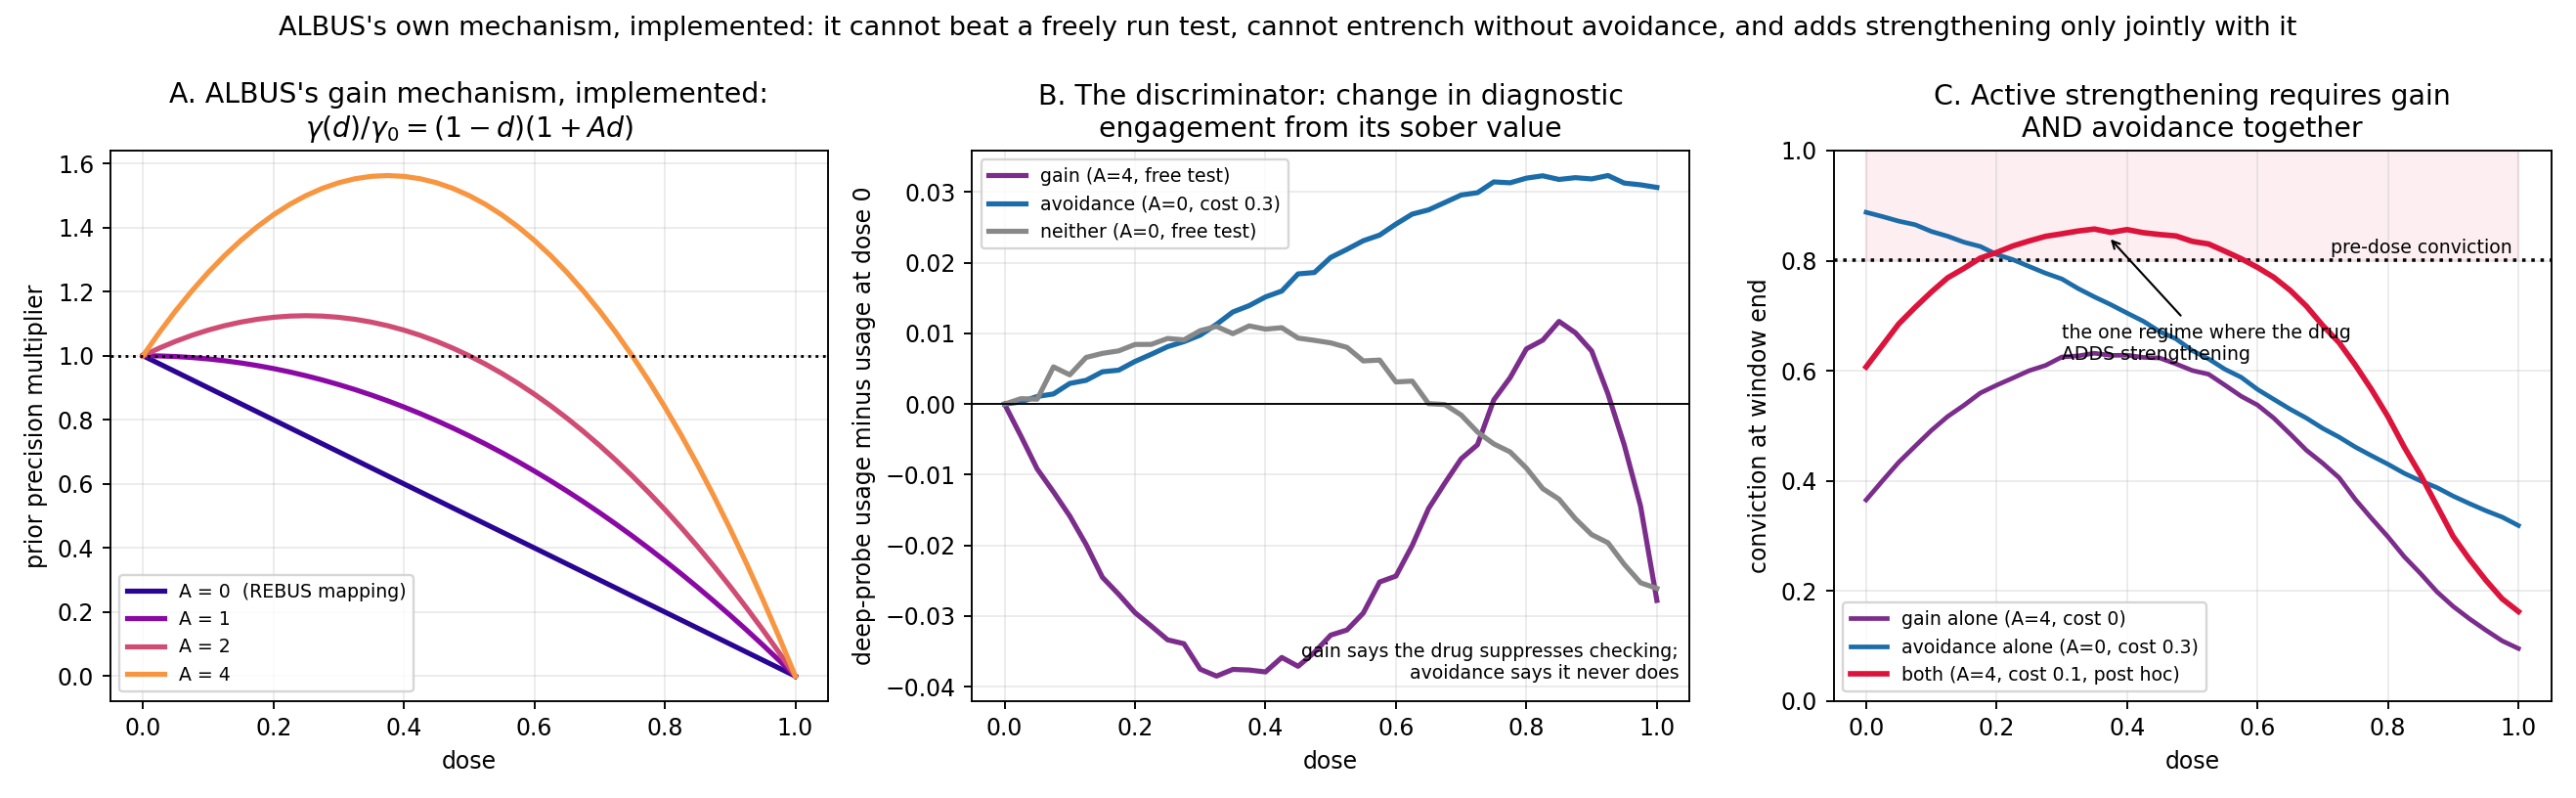
\includegraphics[width=\textwidth]{figure_gain.png}
\caption{Gain versus avoidance. (A) The implemented mapping. (B) The sign
discriminator: gain suppresses diagnostic engagement at low dose, avoidance never
does. (C) Active drug-added strengthening exists only where gain and a modest
test cost combine.}
\label{fig:gain}
\end{figure}

\section{Hierarchy, learning, and interpretive capture}
\label{sec:learning}

The standing objection to consolidation is that active inference already provides
persistence through parameter learning. Amendment 8 (predictions 30 to 33) builds
it: a two-level model with Dirichlet-mean learning on the stored prior and four
increment rules. Learning inherits the fork: dose spread in the lasting outcome
is strictly positive when the increment contains the dose-dependent posterior and
exactly zero when it is computed from evidence alone or from decay. The
underdetermination does not dissolve; it moves into the choice of increment,
which no theory states. A dose-dependent learning rate, the plasticity reading of
psychedelic action, cannot rescue the evidence-driven rule: it scales how far the
belief moves but not where it moves toward (the increment's direction shift
across dose is exactly zero there, against 0.72 and 1.36 under posterior- and
encoding-driven rules). Plasticity and relaxation are dissociable claims:
magnitude change versus content change.

The hierarchy's genuine addition is \textbf{interpretive capture}. With encoding
driven by top-down weighted perception ($\kappa = 3$) in an ambiguous world, the
declared prediction of emergent self-strengthening failed (no cell exceeded the
starting conviction; closest 0.799 against 0.8007) and something better appeared:
the conviction freezes. A 32-fold increase in learning moves lasting conviction
by 0.008 and lasting insight stays at zero, because the rigid prior explains
ambiguous events as conviction-typical and the learning rule counts those
explanations as evidence. Learning is not blocked; it is captured. Dose breaks
the loop from the perception side.

\begin{figure}[t]
\centering
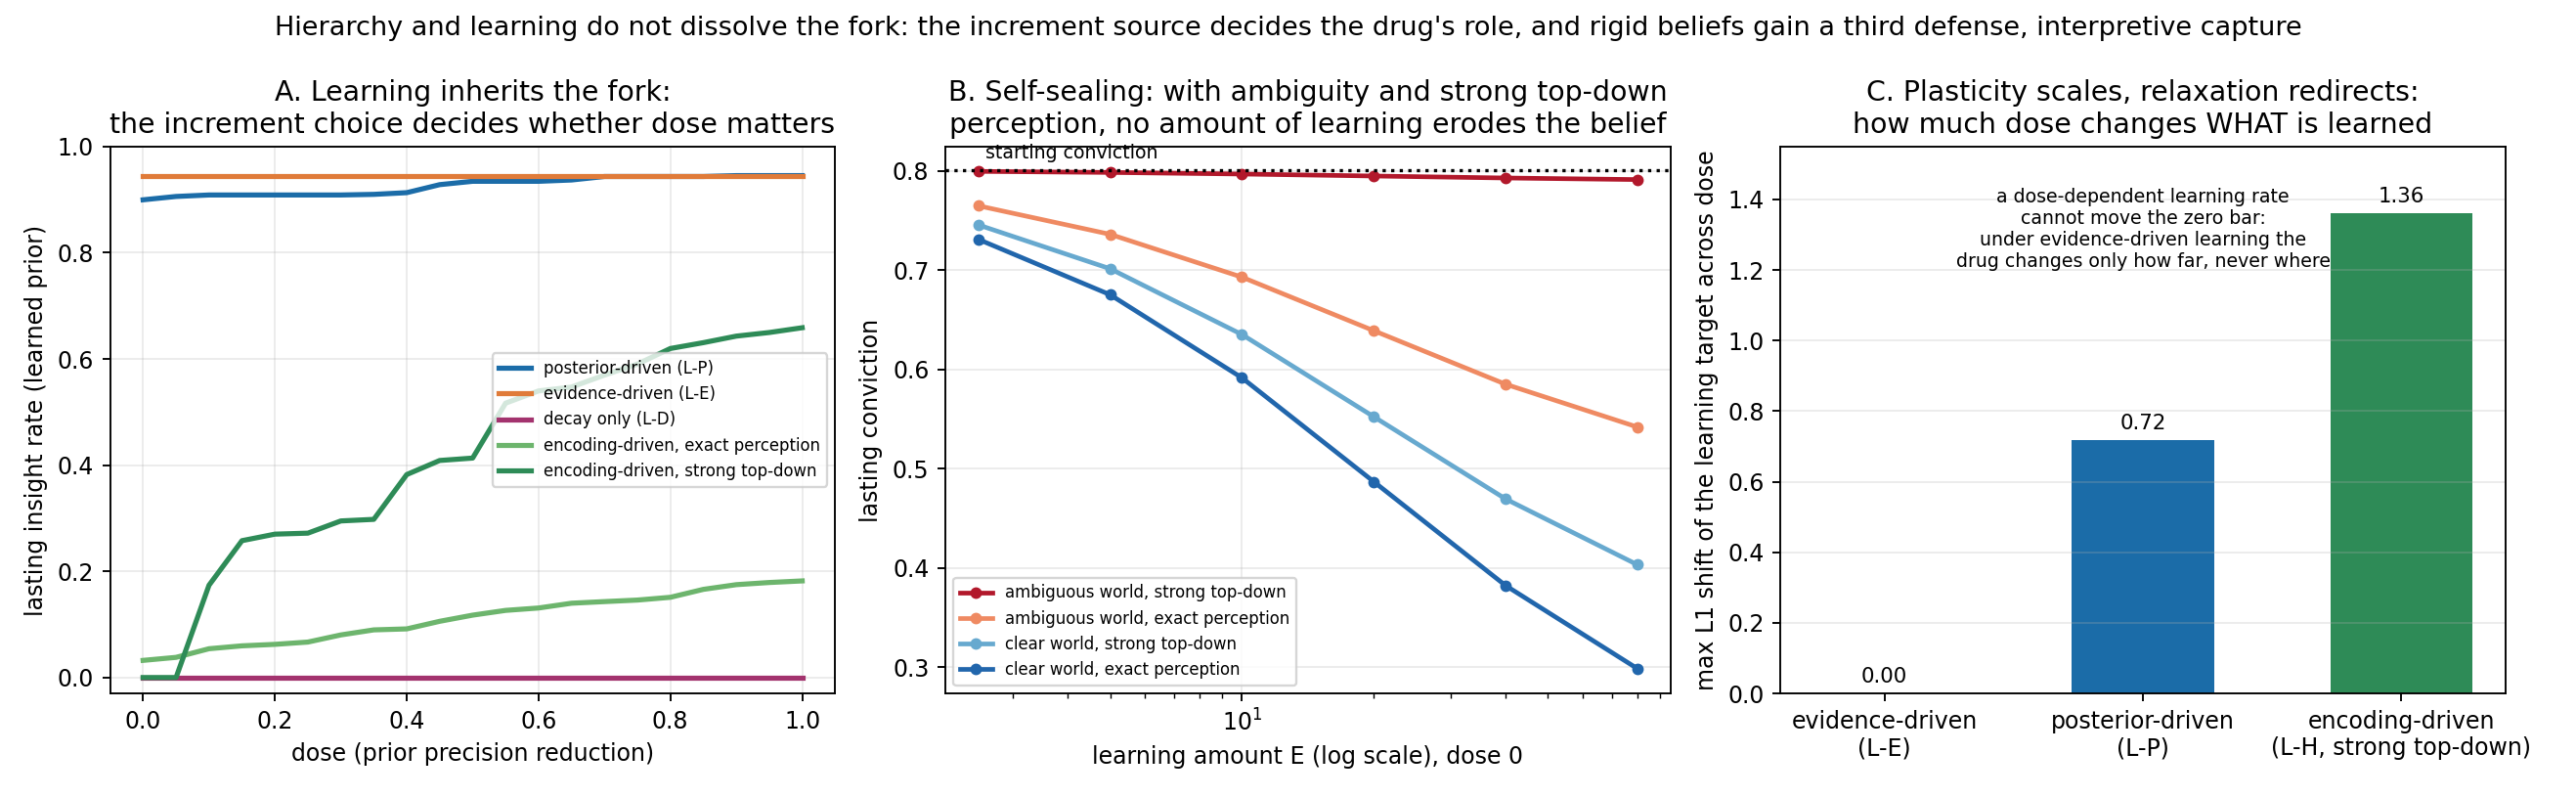
\includegraphics[width=\textwidth]{figure_hierarchy.png}
\caption{Hierarchy and learning. (A) The increment choice decides whether dose
matters; zeros are exact. (B) Self-sealing within a session: under ambiguity and
strong top-down perception, learning amount stops mattering. (C) Plasticity
scales, relaxation redirects.}
\label{fig:hierarchy}
\end{figure}

\section{Sessions: capture is delay, not destiny}
\label{sec:sessions}

Amendment 9 (predictions 34 to 37) runs capture across 40 sessions with an
evolving stored prior, under two count-mass assumptions (fixed mass and Dirichlet
accumulation), against unbiased learning. Most of the declared predictions
failed, and the failures are the findings. The single-session freeze dissolves:
each session leaks a little truth past the biased perception, the leak weakens
the top-down grip, and erosion accelerates, a slow leak then a dam break.
Majority insight arrives by session 8 (fixed mass) or 23 (accumulating), against
3 to 4 for unbiased learning; the declared threefold-delay bar failed, and
neither declared alternative (plateau, climb) occurred. A same-day correction was
issued to the capture writeup: self-sealing is a within-session phenomenon and a
multi-session delay, not destiny, in a stationary world.

The clinically loaded questions land on assumptions no theory states. Under
fixed mass, waiting helps (untreated sessions erode the belief before treatment
starts). Under accumulation, difficulty is non-monotone with a hardest window a
few sessions in, and the hump requires capture and accumulation jointly. At
matched total exposure, protocol shape (one high-dose session versus five
low-dose sessions) moves outcomes by less than a point while the mass assumption
moves them by 35 points. Whether experience rigidifies memory, and whether the
world keeps volunteering disconfirming evidence, carry the answers usually
attributed to the drug.

\begin{figure}[t]
\centering
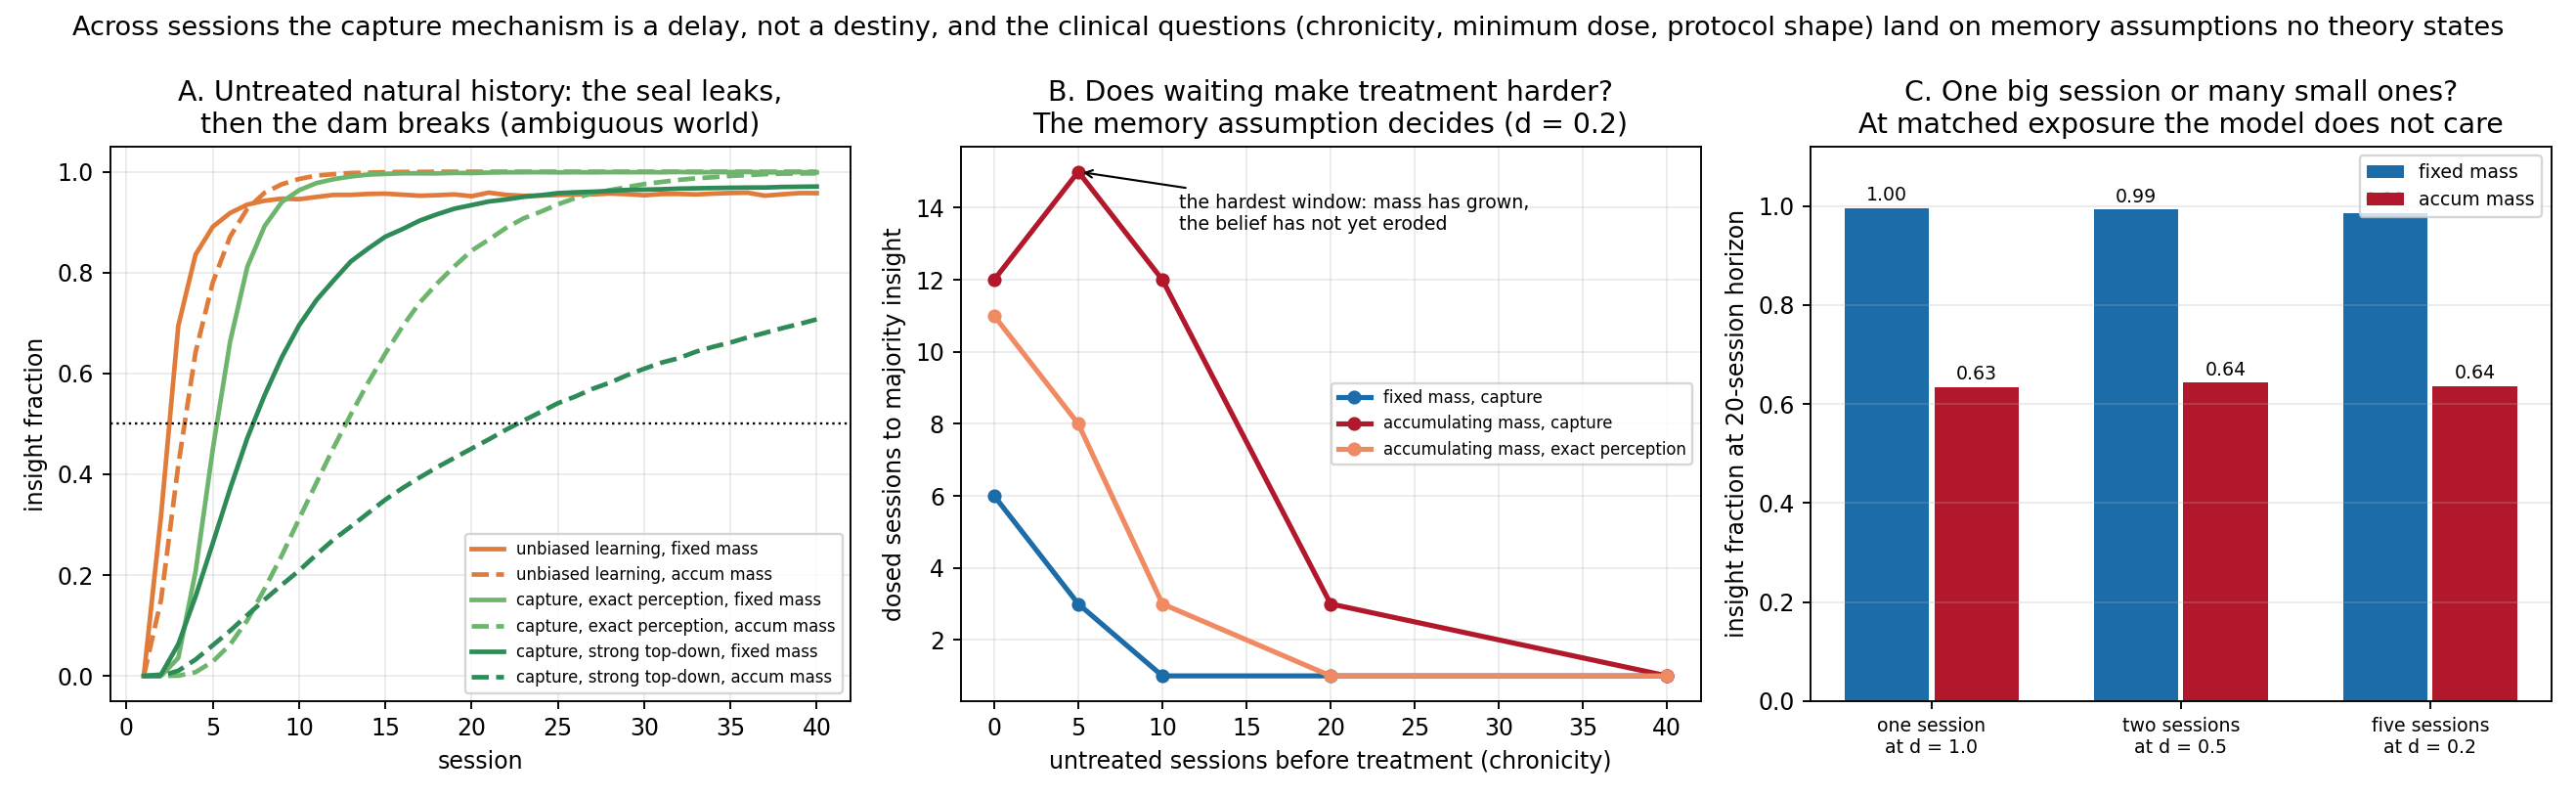
\includegraphics[width=\textwidth]{figure_sessions.png}
\caption{Compounding sessions. (A) Natural history: the seal leaks, then breaks.
(B) Whether chronicity hurts is decided by the memory-mass assumption. (C) At
matched exposure, protocol shape is second-order.}
\label{fig:sessions}
\end{figure}

\section{The ratchet}
\label{sec:ratchet}

The sessions arm's world volunteers evidence; a passive perceiver can distort it
but not refuse it. Avoidance can. Amendment 10 (predictions 38 to 41) composes
the costly-test agent with capture-weighted learning across sessions, and the
loop the earlier arms could not close, closes. At cost 0.3 with capture, stored
conviction climbs from 0.801 to 0.989 and locks; at cost 0.8 it locks at both
perception settings (0.946 and 1.000); insight never arrives. This is the first
permanent entrenchment in the family, produced by dynamics rather than
parameter assumption.

The transient case exposes the mechanism. Without capture, avoidance is
self-limiting: shallow eliminations migrate stored mass onto the confusable pair
jointly, rebuilding exactly the uncertainty that makes the test worth its cost;
diagnostic engagement rises across sessions (0.024 to 0.061), the test gets paid
for, and the belief resolves by session 17. Capture starves that channel: the
doubt is never credited, engagement falls to 0.015 and stays there. Avoidance
loads the trap; capture locks it; high enough cost welds it (engagement 0.000
throughout, both settings).

Treatment then fails three distinct ways. Below the crossover, dosed sessions
never open the test (subthreshold dosing proved useless rather than harmful,
against the declared prediction: untreated natural history already saturates).
At high cost, even maximal dose dissolves conviction to 0.42 and stalls forever
with insight never crossing, the dissolution-without-insight state now terminal:
the test stays priced out at every dose, so nothing discriminating ever arrives.
And chronicity is finally real: at fixed mass, where the previous arm found time
heals, waiting from session 5 to session 20 converts a 12-session cure into
never, and accumulating mass removes the last rescue. Each failure mode has a
distinct signature in the observable the model keeps pointing at: engagement
with the avoided test.

\begin{figure}[t]
\centering
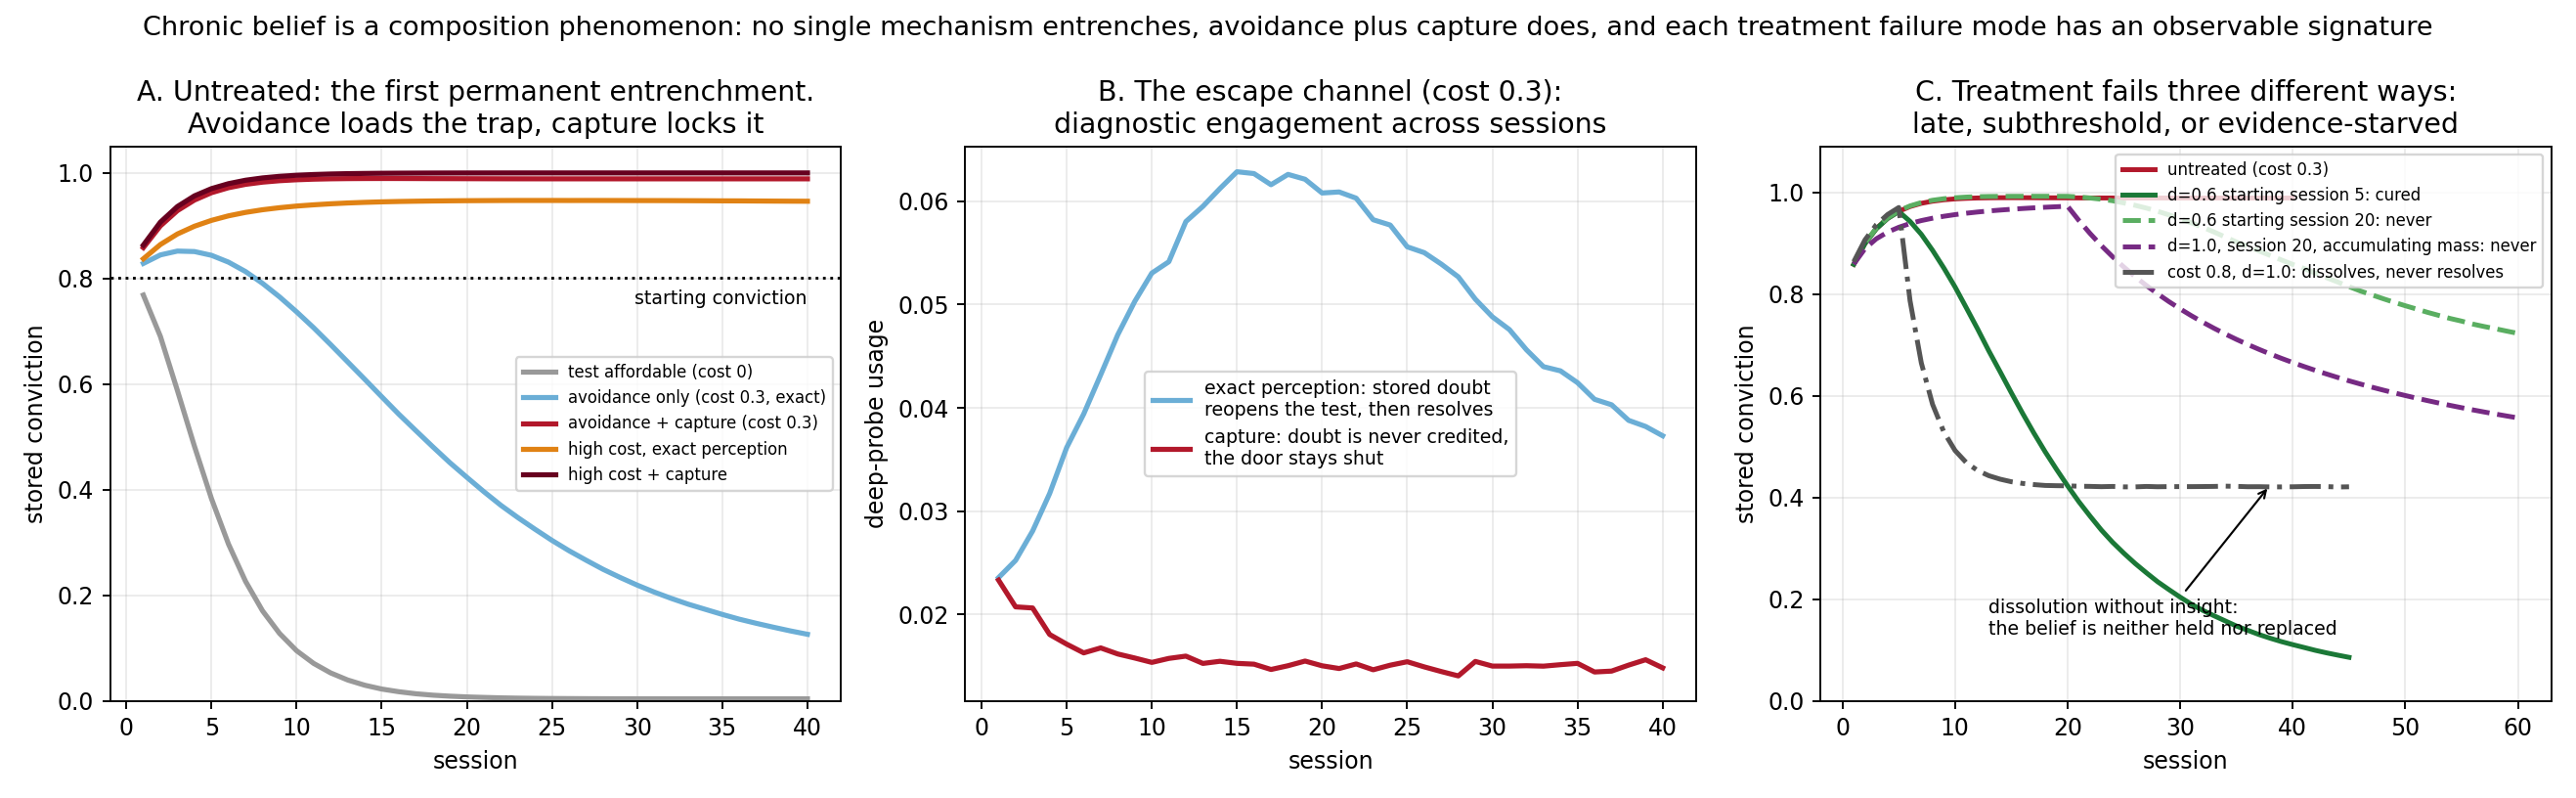
\includegraphics[width=\textwidth]{figure_ratchet.png}
\caption{The ratchet. (A) Untreated natural history: avoidance plus capture is
the first permanent entrenchment. (B) The escape channel: stored doubt reopens
the test unless capture starves it. (C) Three treatment failure modes.}
\label{fig:ratchet}
\end{figure}

\section{Discussion}
\label{sec:discussion}

Read together, the five arms support one sentence: \textbf{in this model family,
psychedelic therapy is precision-modulated exposure.} The drug's derivable role
is to raise the epistemic value of an avoided test until it clears its cost, or
to unfreeze what biased perception encodes; its benefit is gated by dose, cost,
and timing; and chronic belief is what forms when avoidance and biased
interpretation compose, because each disables the other's natural correction.
None of the loop's parts is our discovery: safety behaviors, exposure, and
avoidance-free exposure under psychedelics are established clinical ideas
\cite{salkovskis1991,foakozak1986,craske2014,wolff2020}. The formalization
contributes what verbal accounts cannot fix:

\begin{enumerate}
  \item \textbf{Necessity results.} Precision mechanics alone produce no
  strengthening; gain alone beats no freely run test; capture alone cannot
  prevent recovery; avoidance alone recovers through its own stored doubt.
  Entrenchment requires composition, which is a falsifiable structural claim.
  \item \textbf{A derived drug mechanism} with quantitative signatures: the
  crossover, the ceiling, the dose-zero peak under relaxation-only mappings, and
  the confirmed interior window where gain and avoidance jointly yield active
  strengthening.
  \item \textbf{Discriminating predictions} stated in one observable, diagnostic
  engagement: it rises with dose where therapy works, dips at low dose only
  under the gain account, rises across sessions where recovery is coming,
  and is flat at floor in every untreatable regime. A treatment study that
  measures engagement with avoided disconfirming material as a function of dose
  would test this family directly.
\end{enumerate}

\section{Limitations}
\label{sec:limitations}

The test cost is imposed, not derived; deriving avoidance from aversion to
expected self-model revision is the named next arm, and until then the
untreatable regimes inherit a free parameter. The world is stationary and benign
except where avoidance intervenes; every time-heals result is conditional on
that. The learning rules are a sample of a large space; the capture rule in
particular is one defensible localization of biased encoding. All thresholds are
ordinal claims. Belief dynamics only: no phenomenology, no pharmacology, and the
dissolution-without-insight state must not be over-read clinically. Failed and
half-failed predictions are part of the record throughout (25 above threshold
cost, 32b, the magnitude of 34, the shapes of 35 and 37, the harmful half of
39); two same-day corrections were issued and are preserved in the files rather
than silently amended.

\section{Reproducibility}
\label{sec:repro}

The public repository \url{https://github.com/ArtHangup/rebus-albus-sim}
contains every amendment, all code, all result files, and the git history that
orders each declaration before its implementation (amendments 6 through 10 at
commits \texttt{6d4e093}, \texttt{156c626}, \texttt{ab55a19}, \texttt{3615dd2},
\texttt{ca798a0}; confirmatory amendment 11 at \texttt{27da277}, pushed publicly
before its run). Simulations are pure NumPy with fixed seeds; total API spend
was \$0. Future arms will additionally be preregistered on OSF Registries.

\begin{thebibliography}{99}

\bibitem{rogers2026} J.~Rogers. What the theory never specifies: Preregistered
simulations of REBUS and ALBUS. Preprint, 2026. Code and history:
github.com/ArtHangup/rebus-albus-sim.

\bibitem{carhart2019} R.~L. Carhart-Harris and K.~J. Friston. REBUS and the
anarchic brain: Toward a unified model of the brain action of psychedelics.
\emph{Pharmacological Reviews}, 71(3):316-344, 2019.

\bibitem{safron2025} A.~Safron, A.~Juliani, N.~Reggente, V.~Klimaj, and
M.~Johnson. On the varieties of conscious experiences: Altered beliefs under
psychedelics (ALBUS). \emph{Neuroscience of Consciousness}, 2025(1):niae038, 2025.

\bibitem{salkovskis1991} P.~M. Salkovskis. The importance of behaviour in the
maintenance of anxiety and panic: A cognitive account. \emph{Behavioural
Psychotherapy}, 19(1):6-19, 1991.

\bibitem{foakozak1986} E.~B. Foa and M.~J. Kozak. Emotional processing of fear:
Exposure to corrective information. \emph{Psychological Bulletin}, 99(1):20-35,
1986.

\bibitem{craske2014} M.~G. Craske, M.~Treanor, C.~C. Conway, T.~Zbozinek, and
B.~Vervliet. Maximizing exposure therapy: An inhibitory learning approach.
\emph{Behaviour Research and Therapy}, 58:10-23, 2014.

\bibitem{wolff2020} M.~Wolff, R.~Evens, L.~J. Mertens, M.~Koslowski, F.~Betzler,
G.~Gr\"under, and H.~Jungaberle. Learning to let go: A cognitive-behavioral model
of how psychedelic therapy promotes acceptance. \emph{Frontiers in Psychiatry},
11:5, 2020.

\bibitem{zeifman2020avoid} R.~J. Zeifman, A.~C. Wagner, R.~Watts, H.~Kettner,
L.~J. Mertens, and R.~L. Carhart-Harris. Post-psychedelic reductions in
experiential avoidance are associated with decreases in depression severity and
suicidal ideation. \emph{Frontiers in Psychiatry}, 11:782, 2020.

\bibitem{zeifman2025} R.~J. Zeifman, M.~J. Spriggs, H.~Kettner, T.~Lyons,
F.~E. Rosas, P.~A.~M. Mediano, D.~Erritzoe, and R.~L. Carhart-Harris. From
relaxed beliefs under psychedelics (REBUS) to revised beliefs after psychedelics
(REBAS). \emph{Scientific Reports}, 15:3651, 2025.

\bibitem{corlett2010} P.~R. Corlett, J.~R. Taylor, X.-J. Wang, P.~C. Fletcher,
and J.~H. Krystal. Toward a neurobiology of delusions. \emph{Progress in
Neurobiology}, 92(3):345-369, 2010.

\bibitem{adams2013} R.~A. Adams, K.~E. Stephan, H.~R. Brown, C.~D. Frith, and
K.~J. Friston. The computational anatomy of psychosis. \emph{Frontiers in
Psychiatry}, 4:47, 2013.

\bibitem{sterzer2018} P.~Sterzer, R.~A. Adams, P.~Fletcher, C.~Frith, S.~M.
Lawrie, L.~Muckli, P.~Petrovic, P.~Uhlhaas, M.~Voss, and P.~R. Corlett. The
predictive coding account of psychosis. \emph{Biological Psychiatry},
84(9):634-643, 2018.

\bibitem{powers2017} A.~R. Powers, C.~Mathys, and P.~R. Corlett.
Pavlovian conditioning-induced hallucinations result from overweighting of
perceptual priors. \emph{Science}, 357(6351):596-600, 2017.

\bibitem{rajpal2022} H.~Rajpal, P.~A.~M. Mediano, F.~E. Rosas, et al.
Psychedelics and schizophrenia: Distinct alterations to Bayesian inference.
\emph{NeuroImage}, 263:119624, 2022.

\bibitem{sandved2021} L.~Sandved-Smith, C.~Hesp, J.~Mattout, K.~Friston,
A.~Lutz, and M.~J.~D. Ramstead. Towards a computational phenomenology of mental
action: Modelling meta-awareness and attentional control with deep parametric
active inference. \emph{Neuroscience of Consciousness}, 2021(1):niab018, 2021.

\bibitem{fisher2024} E.~L. Fisher et al. Psilocybin increases optimistic
engagement over time: Computational modelling of behaviour in rats.
\emph{Translational Psychiatry}, 14:394, 2024.

\bibitem{mago2026} J.~Mago et al. Computational spirits: A neuroscientific
account of psychedelic entity encounters. \emph{Neuroscience of Consciousness},
2026(1):niaf069, 2026.

\end{thebibliography}

\end{document}
